%=====================================================================
\chapter{Explainable and Causal Framework}
\label{ch:causal}
%=====================================================================

\textbf{Research Objective 3.} \emph{To establish and evaluate an explainable artificial
intelligence framework capable of delivering transparent and interpretable predictions in stock
selection, analysing the impact of sentiment data noise and exploring the temporal dynamics
between sentiment shifts and stock price movements.}

\vspace{0.4em}
This objective has two halves that are usually pursued separately and are pursued together here.
The first is transparency: making the reasoning behind a stock-selection decision inspectable.
The second is a measurement problem: establishing how much noise the sentiment channel actually
carries and how sentiment shifts relate in time to price movements. They belong together because
an explanation that rests on a noisy input is not an explanation, and because
Chapter~\ref{ch:llm} closed on precisely the question that the second half answers --- whether the
bounded value of the sentiment channel reflects inadequate measurement or genuine absence of
predictability.

The transparency work is reported in Sections~\ref{sec:dchf-design} to~\ref{sec:dchf-perf} and
appears in publication~\pubcite{P2}; the sentiment diagnostics are reported in
Sections~\ref{sec:sent-validity} to~\ref{sec:sent-leadlag} and draw on~\pubcite{P3}
and~\pubcite{P5}.

\section{Transparency at the Level of Structure Rather Than Attribution}
\label{sec:dchf-rationale}

\subsection{What post-hoc attribution can and cannot deliver}

The standard response to model opacity is post-hoc attribution. Given a fitted model and an
input, methods such as Shapley additive explanations~\cite{lundberg2017} or local surrogate
models~\cite{ribeiro2016} report how much each input contributed to the output; language models
can then render that attribution in prose~\cite{koa2024}. These methods are well founded and are
genuinely useful for auditing a deployed system.

Their limitation is structural. Post-hoc attribution is faithful to the \emph{model}: it reports
what the fitted function did. It is silent on whether what the model did corresponds to anything
in the market. A feature that co-moves with the target for entirely spurious reasons receives an
attribution indistinguishable from that of a genuine driver, and an audience shown the resulting
explanation has been given an accurate account of the model and a potentially misleading account
of the world. When the model is subsequently deployed and the spurious relationship breaks, the
explanation will have provided no warning.

\subsection{The alternative pursued here}

This chapter therefore pursues transparency at the level of \emph{structure} rather than of
attribution. The feature set entering the model is constrained, \emph{before any learning takes
place}, to variables with demonstrable directed influence, recovered by conditional independence
testing over lagged series. The explanation available afterwards is not ``the model used feature
$X$'' but ``feature $X$ was admitted because $X$ improves the prediction of the target beyond the
target's own history, and here is the graph''. That statement is auditable by someone who does not
trust the model, which is the property an investment committee or a regulator actually requires.

The trade is stated honestly. Structural transparency constrains the hypothesis space and may
therefore cost accuracy relative to an unconstrained model. Section~\ref{sec:dchf-causal} reports
the offsetting benefit: the causal constraint \emph{retains} relationships that a correlational
filter would have discarded, so in this universe the constraint is not merely a cost.

\section{Design of the Dynamic-Causal Hybrid Framework}
\label{sec:dchf-design}

The framework operates in three sequential stages, shown in Figure~\ref{fig:dchf}.

\begin{figure}[!htb]
\centering
\scalebox{0.88}{\begin{tikzpicture}[node distance=3mm]
\node[blkd,minimum width=100mm,minimum height=7mm] (in)
  {Daily and intraday price series, five NIFTY50 constituents across five sectors};

\node[blk,below=6mm of in,minimum width=100mm,minimum height=12mm] (s1)
  {\textbf{Stage 1 --- causal graph discovery}\\
   conditional independence testing over lagged series $\Rightarrow$ time-varying adjacency
   matrix $A(t)$;\\
   edge $e_{ij}$ retained when $X_i$ improves the prediction of $X_j$ beyond $X_j$'s own past};

\node[blkg,below=5mm of s1,minimum width=100mm,minimum height=13mm] (s2)
  {\textbf{Stage 2 --- multi-scale temporal memory encoding}\\
   parallel recurrent encoders at 1-day, 5-day and 21-day granularity with temporal attention;\\
   $h_t = \mathrm{Debias}\big(\mathrm{Conv}_{1\times k}[\,h^{\text{intraday}}_{t-1},
   h^{\text{daily}}_{t-1}, h^{\text{weekly}}_{t-1}\,]\big)$};

\node[blka,below=5mm of s2,minimum width=100mm,minimum height=12mm] (s3)
  {\textbf{Stage 3 --- credibilistic portfolio optimisation}\\
   returns as triangular fuzzy numbers; range directional measure formulation;\\
   $\max_w \; \big(\mathbb{E}[\tilde{R}] - \lambda\,\mathrm{CVaR}_\alpha(\tilde{R})\big)
   \big/ \mathrm{Entropy}(w)$};

\node[blkd,below=5mm of s3,minimum width=100mm,minimum height=7mm] (out)
  {Sparse, causally traceable portfolio with an auditable feature-selection rationale};

\draw[ar] (in)--(s1); \draw[ar] (s1)--(s2); \draw[ar] (s2)--(s3); \draw[ar] (s3)--(out);
\draw[arb] (s1.west) to[out=180,in=180] node[lbl,left=1mm,align=right]
  {graph refit as\\structure shifts} (s3.west);
\end{tikzpicture}}
\caption[Three-stage Dynamic-Causal Hybrid Framework]{Three-stage Dynamic-Causal Hybrid
Framework. Causal discovery constrains the feature set, multi-granularity encoding captures
structure at several horizons, and credibilistic optimisation converts the signal into holdings
under epistemic uncertainty.}
\label{fig:dchf}
\end{figure}

\subsection{Stage 1: causal graph discovery}

Let $G_t = (V, E_t)$ be the causal graph at session $t$ over $N$ instruments. A directed edge
$e_{ij} \in E_t$ is retained when series $X_i$ improves the prediction of series $X_j$ beyond
what $X_j$'s own history achieves, tested by conditional independence over lagged closing-price
series following the constraint-based procedure of Section~2.8.2~\cite{spirtes2000,granger1969}.
The result is a time-varying adjacency matrix $A(t)$ whose entry $(i,j)$ records the strength of
the directed influence of instrument $i$ on instrument $j$.

The graph is refitted as structure shifts rather than estimated once. This is the direct response
to the limitation of static causal formulations identified in Section~3.3.2: a static graph cannot
represent the structural breaks produced by Union Budget or monetary policy announcements, which
in the Indian market reset inter-instrument relationships within hours.

\subsection{Stage 2: multi-scale temporal memory encoding}

Financial series carry structure at several time scales at once, a property consistent with the
fractal description of market dynamics and with the multi-granularity architectures reviewed in
Section~3.3.3. Three parallel recurrent encoders therefore process short (1-day), medium (5-day)
and long (21-day) horizons, and their hidden states are combined through a convolutional temporal
attention layer with a debiasing correction,
\begin{equation}
h_t = \mathrm{Debias}\!\left(\mathrm{Conv}_{1\times k}
\left[h^{\text{intraday}}_{t-1},\, h^{\text{daily}}_{t-1},\, h^{\text{weekly}}_{t-1}\right]\right),
\label{eq:mtmd}
\end{equation}
where $k$ is the kernel size. The purpose of the multi-scale construction is separation:
volatility clustering operates at one scale and momentum at another, and an encoder that sees only
one scale cannot distinguish a genuine trend from the low-frequency component of a
volatility cycle.

The debiasing term carries an assumption that Section~\ref{sec:dchf-perf} reports failing
empirically, and it is flagged here rather than after the fact. The correction assumes
\emph{stationary} noise properties, so that a bias estimated on earlier data remains valid later.
Indian market volatility is not stationary.

\subsection{Stage 3: credibilistic portfolio optimisation}

The third stage converts the encoded signal into holdings. Rather than forcing a point estimate
of expected return that the data do not support, returns are represented as triangular fuzzy
numbers $[l, m, u]$, which admit vagueness in the market view explicitly --- the epistemic
uncertainty of Section~2.4.2, expressed in a possibilistic rather than probabilistic
formalism. Weights are then obtained by
\begin{equation}
\max_{w}\ \frac{\mathbb{E}[\tilde{R}] - \lambda\,\mathrm{CVaR}_{\alpha}(\tilde{R})}
{\mathrm{Entropy}(w)}
\qquad \text{subject to } w \in \text{RDM-DEA feasible set},
\label{eq:credibilistic}
\end{equation}
following the range directional measure formulation of Kumar and Yadav~\cite{kumar2024rdmdea},
which handles positive and negative returns without assuming normality. The entropy denominator
penalises concentration, and the conditional value at risk term penalises tail exposure rather
than variance, which is the appropriate risk measure when the return distribution is asymmetric.

The coupling of Equation~\eqref{eq:credibilistic} to a \emph{dynamic} causal graph is the
extension this framework contributes: Kumar and Yadav's formulation rebalances at fixed intervals,
whereas here the feasible set is reconstructed when the causal structure shifts.

\section{Experimental Setup}
\label{sec:dchf-setup}

Data were obtained for five NIFTY50 constituents chosen to span five sectors: RELIANCE (energy
and conglomerate), TCS (information technology), TITAN (consumer discretionary), NESTLEIND
(fast-moving consumer goods) and HDFCBANK (financials). The period is 1~January 2024 to
31~March~2025, comprising 308 trading sessions.

The universe is deliberately small, and the reason is computational rather than methodological.
Constraint-based causal discovery requires a number of conditional independence tests that grows
combinatorially with the number of variables, so a five-instrument universe is tractable and a
fifty-instrument universe is not with the same procedure. Section~\ref{sec:dchf-limits} treats
scalable discovery as the principal open problem of this chapter. The five names were selected for
sectoral spread and liquidity rather than by any performance criterion, which matters because
selecting instruments on outcomes would invalidate the graph.

Evaluation is against a passive buy-and-hold benchmark over the same window, with the causal
structure, the recovered graph density and the behaviour around the 2024 Union Budget examined as
separate diagnostics.

\section{Results: Causal Structure as an Explanation Mechanism}
\label{sec:dchf-causal}

\subsection{The recovered graph}

Table~\ref{tab:causal} reports the recovered adjacency matrix over the 308-session window.

\begin{table}[!htb]
\centering
\caption[Dynamic causal adjacency matrix]{Dynamic causal adjacency matrix $A(t)$ over five
NIFTY50 constituents, January 2024 to March 2025. Entry $(i,j)$ is the strength of the directed
influence of row $i$ on column $j$.}
\label{tab:causal}
\tabfont
\begin{tabular}{@{}lrrrrr@{}}
\toprule
\textbf{Influencing $\downarrow$ / Influenced $\rightarrow$} & \textbf{HDFCBANK} &
\textbf{NESTLEIND} & \textbf{RELIANCE} & \textbf{TCS} & \textbf{TITAN} \\
\midrule
HDFCBANK  & 1.000 & 0.299 & 0.791 & 0.079 & 0.460 \\
NESTLEIND & 0.072 & 1.000 & 0.356 & 0.130 & 0.006 \\
RELIANCE  & \textbf{0.913} & 0.324 & 1.000 & \textbf{0.650} & \textbf{0.849} \\
TCS       & 0.110 & 0.670 & 0.516 & 1.000 & 0.436 \\
TITAN     & 0.337 & 0.058 & 0.216 & 0.610 & 1.000 \\
\bottomrule
\end{tabular}
\end{table}

The graph has a density of 0.850 and a maximum causal score of 1.000, indicating strong directed
interdependence among the constituents --- unsurprising in an index whose members share
macroeconomic exposure, but the \emph{asymmetry} of that interdependence is informative.

\subsection{A systematic causal hub}

The most interpretable feature of Table~\ref{tab:causal} is the RELIANCE row. It exerts strong
directed influence on HDFCBANK (0.913), TITAN (0.849) and TCS (0.650), while the corresponding
column shows markedly weaker influence received in return: 0.791 from HDFCBANK, 0.216 from TITAN,
0.516 from TCS, 0.356 from NESTLEIND. Outgoing influence systematically exceeds incoming
influence, which is the signature of a causal hub.

Figure~\ref{fig:graph} renders the structure above an edge threshold of 0.3.

\begin{figure}[!htb]
\centering
\scalebox{0.88}{\begin{tikzpicture}[node distance=20mm,
  nd/.style={circle,draw=black!70,fill=blue!6,minimum size=14mm,font=\scriptsize,align=center},
  hub/.style={circle,draw=black!80,fill=orange!22,minimum size=16mm,font=\scriptsize\bfseries,align=center},
  ce/.style={-{Latex[length=1.6mm,width=1.2mm]},draw=black!60},
  cs/.style={-{Latex[length=1.9mm,width=1.5mm]},draw=black!85,line width=1.0pt}]
\node[hub] (rel) at (0,0) {RELI-\\ANCE};
\node[nd] (hdfc) at (-34mm,15mm) {HDFC\\BANK};
\node[nd] (tcs) at (34mm,15mm) {TCS};
\node[nd] (titan) at (-26mm,-22mm) {TITAN};
\node[nd] (nest) at (28mm,-22mm) {NESTLE\\IND};

\draw[cs] (rel) -- node[lbl,above,sloped,font=\tiny] {0.913} (hdfc);
\draw[cs] (rel) -- node[lbl,above,sloped,font=\tiny] {0.849} (titan);
\draw[cs] (rel) -- node[lbl,above,sloped,font=\tiny] {0.650} (tcs);
\draw[ce] (hdfc) to[bend left=14] node[lbl,above,sloped,font=\tiny] {0.791} (rel);
\draw[ce] (hdfc) to[bend right=28] node[lbl,left,font=\tiny] {0.460} (titan);
\draw[ce] (tcs) to[bend left=18] node[lbl,right,font=\tiny] {0.670} (nest);
\draw[ce] (tcs) to[bend left=10] node[lbl,below,sloped,font=\tiny] {0.516} (rel);
\draw[ce] (titan) to[bend right=16] node[lbl,below,font=\tiny] {0.610} (tcs);
\draw[ce] (nest) to[bend left=12] node[lbl,below,sloped,font=\tiny] {0.356} (rel);
\node[lbl,below=4mm of titan,align=left,xshift=10mm]
  {Graph density 0.850; edges shown for strength $>0.3$.\\
   Bold edges mark the causal hub, whose outgoing\\ influence exceeds its incoming influence.};
\end{tikzpicture}}
\caption[Dynamic causal graph recovered from NIFTY50 constituents]{Dynamic causal graph recovered
from NIFTY50 constituent series. The structure is readable, which is the property that makes the
feature selection auditable.}
\label{fig:graph}
\end{figure}

The readability of Figure~\ref{fig:graph} is the point of the exercise. An analyst can inspect it,
compare it against a prior belief about how the Indian market transmits shocks, and reject it if
it conflicts. That is a different kind of object from a bar chart of attribution scores over a
fitted model's inputs, and it is what structural transparency delivers.

\subsection{Correlation and causality diverge, and the divergence is exploitable}

The decisive evidence for the approach is the comparison between correlation and causality. Pairs
exist in this universe --- the influence of RELIANCE on TITAN being the clearest --- for which the
directed causal strength is high (0.849) while the linear correlation between the two series is
low.

The mechanism is unsurprising once stated: influence that operates with a lag, or through a
nonlinear channel such as an input-cost pass-through, does not produce contemporaneous linear
co-movement. The consequence for modelling is decisive. A correlation-based feature selector
applied to this universe would have discarded the RELIANCE--TITAN relationship as uninformative,
and would have done so silently.

This is the mechanistic justification for the framework, and it settles a question that is usually
treated as a trade-off. Transparency and accuracy are commonly presented as opposed: one accepts a
simpler, more interpretable model and pays for it in performance. In this universe they are not
opposed, because the causal constraint \emph{retains} information that the correlational
alternative destroys. The interpretable feature set is a superset of the correlational one along
the dimension that matters.

\section{Performance and the Failure of Stationary Debiasing}
\label{sec:dchf-perf}

Performance over the 308-session window is reported in full, including the respects in which the
framework underperforms.

\begin{table}[!htb]
\centering
\caption[Performance of the Dynamic-Causal Hybrid Framework]{Performance of the Dynamic-Causal
Hybrid Framework over 308 trading sessions, January 2024 to March 2025}
\label{tab:dchf-perf}
\tabfont
\begin{tabular}{@{}L{6.4cm}L{3.0cm}L{4.6cm}@{}}
\toprule
\textbf{Measure} & \textbf{Value} & \textbf{Reading} \\
\midrule
Causal graph density & 0.850 & Strong directed interdependence among constituents \\
Maximum causal score & 1.000 & At least one relationship of maximal measured strength \\
Sharpe ratio & 0.377 & Positive risk-adjusted return over the window \\
Win rate & 48.8\% & Below one half; combined with a positive Sharpe ratio this indicates
asymmetric profit capture \\
Performance against buy-and-hold & $-$8.95\% & Underperformance during a strong bull market \\
Peak volatility, 2024 Union Budget window & 77.67\% & Debiasing layer fails when the noise
process changes \\
\bottomrule
\end{tabular}
\end{table}

\subsection{Asymmetric profit capture}

A win rate below one half combined with a positive Sharpe ratio is not a contradiction; it is the
signature of asymmetric profit capture, in which winning trades are larger than losing ones. The
framework loses more often than it wins and still earns a positive risk-adjusted return, which
means its position sizing is doing work that its directional accuracy is not. Transaction costs
and signal lag account for the nominal shortfall against the passive benchmark.

The honest characterisation is therefore that this is a \emph{capital-preservation} instrument
rather than a return-maximising one, and it underperformed a rising market by 8.95 per cent over a
window in which the market rose strongly. A framework that de-risks on structural signals will
underperform during an uninterrupted advance, which is a property of the design rather than a
defect in its implementation --- but it is a property a practitioner must be told about in
advance, and stating it is part of the contribution. The same characterisation recurs in
Chapter~\ref{ch:allocation} on a much longer sample, where the window includes the crises that
this fifteen-month window does not.

\subsection{The debiasing layer fails when the noise process changes}

The most useful negative result in this chapter is the 77.67 per cent peak volatility recorded
during the 2024 Union Budget announcement window. The debiasing correction in
Equation~\eqref{eq:mtmd} assumes stationary noise properties, and a budget announcement is
precisely an event at which the noise process changes character discretely: volatility clusters
tighten, cross-instrument correlations jump, and the relationship between realised and expected
dispersion breaks.

The result is diagnostic rather than fatal, and it is reported because it identifies a specific,
addressable weakness rather than a general limitation. A debiasing layer whose noise model is
itself state-dependent --- estimating the correction separately within identified market states,
or allowing its parameters to follow the volatility process --- is the direct remedy, and it is
listed as future work in Chapter~\ref{ch:conclusion}. The general lesson generalises beyond this
framework: any correction calibrated on historical noise will be least reliable at exactly the
moments when the noise changes, which are the moments that determine a drawdown.

\section{Sentiment Noise: Construct Validation Against External Evidence}
\label{sec:sent-validity}

The second half of Research Objective~3 concerns how noisy the sentiment channel is. This section
and the two that follow treat that as a measurement problem with three instruments.

\subsection{The claim to be tested}

Naming a series a ``sentiment measure'' is a claim, and it is testable independently of whether
the series makes money. The two questions are routinely conflated in the literature: a sentiment
measure that fails to predict returns is described as a poor measure, and one that predicts
returns is described as validated. Neither inference is sound. A measure can be an accurate
gauge of market sentiment and still fail to forecast returns, if sentiment is priced
contemporaneously; and a measure can forecast returns for reasons unrelated to sentiment.

The construct examined here is a market-derived composite in the tradition of Baker and
Wurgler~\cite{bakerwurgler2007}, built from exchange turnover and dispersion rather than from
text. The reason it is market-derived rather than textual is structural and was stated in
Section~3.2.3: instrument-level, time-stamped news corpora do not exist for the broad index
instruments over which the cross-sectional study of Chapter~\ref{ch:allocation} operates. The
consequence for interpretation is important and is stated again in Section~\ref{sec:sent-predict}.

\subsection{Validation against four independently published series}

The composite was compared against four independently published series, \emph{none} of which
enters the framework at any stage: a household survey of consumer sentiment, an implied volatility
index, a financial stress index and a financial conditions index. Two of these are survey-based or
policy-institution constructions and share no inputs with the composite at all.
Table~\ref{tab:sentval} and Figure~\ref{fig:sent}(a) report the outcome.

\begin{table}[!htb]
\centering
\caption[Validation of the sentiment composite against external series]{Validation of the
market-derived sentiment composite against four independently published series, in levels and in
first differences, over 4,689 sessions from January 2008 to August 2026}
\label{tab:sentval}
\tabfont
\begin{tabular}{@{}L{4.6cm}cL{1.6cm}rrrr@{}}
\toprule
\textbf{External series} & \textbf{Expected sign} & \textbf{Freq.} &
\textbf{$r$ (levels)} & \textbf{$p$} & \textbf{$r$ (diffs)} & \textbf{$p$} \\
\midrule
Household consumer sentiment survey & $+$ & M & $+0.262$ & 0.056 & $+0.240$ & 0.0004 \\
Implied volatility index & $-$ & D & $-0.541$ & 0.0003 & $-0.112$ & 0.0025 \\
Financial stress index & $-$ & W & $-0.606$ & 0.0067 & $-0.254$ & 0.0002 \\
Financial conditions index & $-$ & W & $-0.513$ & 0.0140 & $-0.123$ & 0.0291 \\
\bottomrule
\multicolumn{7}{@{}l@{}}{\scriptsize All four carry the expected sign; all four are significant
in first differences at the five per cent level.}
\end{tabular}
\end{table}

\begin{figure}[!htb]
\centering

\includegraphics[width=0.98\linewidth]{figs/f_sentiment_diag.pdf}
\caption[Sentiment composite diagnostics]{Sentiment diagnostics. (a) Correlation of the sentiment
composite with four independently published series in levels and first differences. (b) The
composite evaluated by identified market state; the states are labelled by fitted volatility and
the composite plays no part in fitting them.}
\label{fig:sent}
\end{figure}

Every correlation carries the expected sign --- positive against the consumer survey, negative
against the three stress and volatility measures --- and every one is significant in first
differences at the five per cent level. Testing in first differences is the more demanding
comparison, because two series that both trend will correlate in levels for reasons unrelated to
their content.

The survey comparison is the informative one. A correlation of $+0.240$ between monthly
\emph{changes} in a composite built from exchange turnover and dispersion, and monthly changes in
what households report to an interviewer, cannot be a mechanical artefact of shared construction:
the two objects have no common input. Either both are measuring a shared latent state, or the
agreement is coincidence, and the significance level makes coincidence implausible.

\subsection{Stability across sub-periods}

A validation that holds only in aggregate may reflect a single episode. The comparison was
therefore repeated within four sub-periods, giving sixteen series-by-sub-period cells.
Figure~\ref{fig:sentstab} reports them.

\begin{figure}[!htb]
\centering
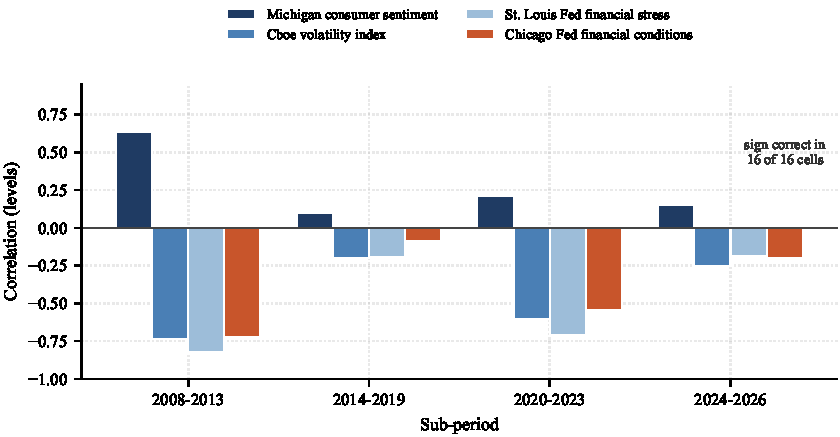
\includegraphics[width=0.92\linewidth]{figs/f_sent_stability.pdf}
\caption[Sub-period stability of the sentiment composite]{Correlation of the sentiment composite
with each of the four external series within four sub-periods. The sign is correct in all sixteen
cells, and magnitudes are largest in the crisis sub-periods, which is the expected pattern for a
stress-sensitive measure.}
\label{fig:sentstab}
\end{figure}

The sign is correct in \emph{all sixteen} cells. The magnitudes are far from constant --- they are
largest in the 2008--2013 and 2020--2023 sub-periods and weakest in the calm 2014--2019 stretch ---
but that variation is itself the expected pattern for a stress-sensitive measure: a gauge of market
anxiety should co-move most strongly with other anxiety measures when there is anxiety to measure,
and should be comparatively uninformative when there is not.

\section{Separation Across Identified Market States}
\label{sec:sent-regime}

A second and independent test is available. If the latent states identified by the regime model of
Chapter~\ref{ch:allocation} are states of \emph{sentiment} as well as of volatility, the composite
should differ systematically across them. The test has force because the mixture model is fitted on
realised volatility and short-horizon momentum, and the sentiment composite is \emph{not} among its
inputs: any separation is separation on a withheld variable.

Table~\ref{tab:sentregime} and Figure~\ref{fig:sent}(b) report the result.

\begin{table}[!htb]
\centering
\caption[Sentiment composite by identified market state]{Mean sentiment composite by identified
market state, with the state labels assigned by ascending fitted volatility. The composite takes
no part in fitting the states.}
\label{tab:sentregime}
\tabfont
\begin{tabular}{@{}L{3.4cm}rrrL{5.4cm}@{}}
\toprule
\textbf{Identified state} & \textbf{$n$} & \textbf{Mean} & \textbf{SD} & \textbf{Test statistic} \\
\midrule
Calm & 160 & $+0.073$ & 0.407 & \multirow{3}{5.4cm}{One-way ANOVA:
$F = 19.34$, $p = 1.8\times10^{-8}$. \\ Kruskal--Wallis: $H = 29.54$,
$p = 3.9\times10^{-7}$.} \\
Transitional & 56 & $-0.140$ & 0.382 & \\
Stress & 7 & $-0.831$ & 0.735 & \\
\bottomrule
\end{tabular}
\end{table}

The ordering is monotone and steep: $+0.073$ in the calm state, $-0.140$ in the transitional
state and $-0.831$ in the stress state. One-way analysis of variance gives $F = 19.34$ with
$p = 1.8 \times 10^{-8}$. Because the stress state contains only seven observations, the
rank-based Kruskal--Wallis test was also computed as a distribution-free check and gives
$H = 29.54$ with $p = 3.9 \times 10^{-7}$; the two agree, so the result does not depend on the
normality assumption that the small stress sample would strain.

The conclusion supported is specific: the identified states may reasonably be described as
\emph{sentiment-and-volatility} states rather than volatility states alone. This matters for the
allocation framework of Chapter~\ref{ch:allocation}, because a regime-conditional risk budget is
more defensible if the regimes correspond to something an investor would recognise.

\section{Predictive Content, Measured Separately}
\label{sec:sent-predict}

The construct is validated. The separate question is whether it forecasts returns, and the answer
is that it does not.

Measured as a cross-sectional information coefficient against next-session returns, the predictive
content of the validated composite over the full multi-asset sample is $-0.026$ with a Newey--West
$t$ statistic of $-2.26$: significantly \emph{negative} rather than positive, and small.
Chapter~\ref{ch:allocation} reports the full set of these measurements, examines whether the
negative relationship is stable enough to exploit by inversion, and finds that it is not.

Three points follow, and keeping them apart is the methodological contribution of this section.

\textbf{A valid measure need not be a profitable one.} A composite can track market sentiment
accurately --- as the sixteen-of-sixteen sign agreement and the $p = 1.8\times10^{-8}$ state
separation establish --- and still fail to forecast returns. If sentiment is incorporated into
prices contemporaneously, an accurate contemporaneous gauge of sentiment will have no forward
information by construction. The two findings are not in tension; they are answers to different
questions.

\textbf{Conflating the two is a recurring error.} A study that reports only the predictive null
invites the reading that the sentiment construct is poor. A study that reports only the validation
invites the reading that sentiment is useful for forecasting. Reporting both is what allows the
correct inference: the measurement is sound and the forward predictability is absent at this
horizon on this universe.

\textbf{The null is about this proxy, not about textual sentiment.} The composite tested here is
market-derived. The bounded but positive findings of Chapter~\ref{ch:llm} concern
language-model-extracted \emph{textual} sentiment on single names with dense news coverage. These
are different constructs measured on different universes, and the null reported here does not
transfer to the other. Section~\ref{sec:sent-answer} returns to what this means for the question
Chapter~\ref{ch:llm} left open.

\section{Sentiment-to-Price Temporal Dynamics}
\label{sec:sent-leadlag}

The final component of Research Objective~3 concerns the temporal relationship between sentiment
shifts and price movements. Three findings, drawn together from the diagnostics of
Chapter~\ref{ch:llm} and the present chapter, characterise it.

\textbf{Spikes precede moves, but the mapping is not simple.} The temporal overlay of sentiment
against price reported in Section~\ref{sec:llm-distribution} shows that strong sentiment spikes
frequently precede major price changes. A simple causal ordering does not follow, because the
relationship between magnitude and direction is not monotone.

\textbf{Two distinct incorporation regimes.} Sustained positive sentiment accompanies gradual
price advances, whereas sharp negative sentiment spikes accompany abrupt declines. Favourable
information is incorporated by accumulation; adverse information by discrete repricing. The two
operate on different timescales, which is a direct argument for the multi-granularity encoder of
Equation~\eqref{eq:mtmd}: a single-horizon model must choose which of the two dynamics to
represent.

\textbf{The channel is genuinely noisy, and the noise is measurable.} The approximately symmetric
sentiment distribution with moderate tails reported in Section~\ref{sec:llm-distribution}
establishes that the extraction pipeline captures real variation rather than producing a biased
categorical output. The information-coefficient measurement of Section~\ref{sec:sent-predict}
establishes that the forward-looking content of the market-derived composite is not
distinguishable from zero in a usable direction. Together these say that the sentiment channel is
measurable, real, and at this horizon largely contemporaneous with price rather than leading it in
a way that can be traded.

\section{Answering the Question Chapter~\ref{ch:llm} Left Open}
\label{sec:sent-answer}

Chapter~\ref{ch:llm} closed by posing a fork. The bounded value of the sentiment channel at a
single-name daily horizon admits two explanations: either the \emph{measurement} is inadequate, in
which case a better extraction pipeline should recover a larger edge; or the measurement is sound
and the \emph{predictability} is not there at that horizon.

The diagnostics of this chapter resolve the fork for the market-derived composite. The construct is
demonstrably sound: correct sign against four independent external series, correct sign in all
sixteen series-by-sub-period cells, and separation across withheld-variable market states at
$p = 1.8 \times 10^{-8}$. Its forward predictive content is separately measured and is not usable.
The limitation is therefore \emph{not} one of measurement. Building a better gauge of the same
construct would not produce a forecast.

The consequence for the thesis is the one stated at the end of Chapter~\ref{ch:llm} and acted upon
in Chapter~\ref{ch:allocation}. If the signal channel is bounded and the boundedness does not stem
from poor measurement, then the framework must earn its value somewhere other than the signal
layer. The natural candidate is the decision layer, where the same information can be used to
determine \emph{how much risk to carry} rather than \emph{which assets to hold}. That hypothesis is
tested directly, with a matched-exposure ablation designed to distinguish the two, in the next
chapter.

One qualification is restated so that it is not lost. This resolution applies to the
market-derived composite on a broad-instrument universe. It does not close the question for
textual sentiment on instruments with dense, time-stamped news coverage, where
Chapter~\ref{ch:llm} found a small but real and orthogonal signal. Applying the fusion hypothesis
where such a corpus exists would convert a proxy null into a genuine test, and this is identified
as the first item of future work in Chapter~\ref{ch:conclusion}.

\section{Limitations}
\label{sec:dchf-limits}

Four limitations bound this chapter.

\textbf{Five instruments, not fifty.} Constraint-based causal discovery scales combinatorially in
the number of variables, so the recovered graph covers five constituents over fifteen months.
Whether the hub structure identified here persists across the full index, and whether it is stable
across longer periods, is not established. Scalable causal discovery is the principal open problem.

\textbf{Predictive precedence, not intervention.} The notion of causality used is the operational
one of Section~2.8.1: $X$ improves the prediction of $Y$ beyond $Y$'s own past. This is not
interventional identification, and no claim is made that acting on $X$ would move $Y$. Confounding
by an unobserved common driver --- a macroeconomic shock that moves both instruments with
different lags --- is not excluded by the procedure.

\textbf{Stationary debiasing.} The failure documented in Section~\ref{sec:dchf-perf} is a
limitation of the present implementation rather than of multi-scale encoding in general, and the
remedy is identified.

\textbf{No attribution experiments.} Transparency here rests on structure. Shapley additive
explanations and local surrogate models are reviewed and cited but are not run, so the thesis makes
no comparative claim about structural versus attributional transparency; it argues for the former
on the grounds given in Section~\ref{sec:dchf-rationale} and demonstrates that in this universe it
is not purchased at the cost of information.

\section{Summary}

This chapter pursued transparency at the level of structure rather than attribution, and treated
sentiment noise as a measurement problem rather than an assumption.

The Dynamic-Causal Hybrid Framework constrains the feature set by directed causal structure
recovered through conditional independence testing, encodes intraday, daily and weekly horizons
through a multi-scale memory layer, and allocates through a credibilistic optimiser that admits
vagueness in the market view. Over 308 NIFTY50 sessions it recovers a causal graph of density
0.850 with an identifiable causal hub whose outgoing influence systematically exceeds its
incoming influence, and it demonstrates that strong directed causal influence can coexist with
weak linear correlation --- so that a correlational feature selector would have discarded a
genuine driver. Performance is reported in full: a Sharpe ratio of 0.377 with a win rate of 48.8
per cent, indicating asymmetric profit capture, and an 8.95 per cent shortfall against
buy-and-hold in a rising market, which characterises the framework as a capital-preservation
instrument. The 77.67 per cent peak volatility during the 2024 Union Budget window identifies
stationary debiasing as a specific, addressable weakness.

Sentiment noise was quantified rather than assumed. The composite carries the expected sign
against four independently published series, is significant in first differences against all
four, holds the correct sign in all sixteen series-by-sub-period cells, and separates the
identified market states at $p = 1.8 \times 10^{-8}$ on a variable withheld from the fitting
procedure. Its forward predictive content, measured separately, is not usable. Keeping construct
validity and predictive usefulness apart resolves the question Chapter~\ref{ch:llm} left open: the
limitation is not one of measurement, and the value of the system must therefore be sought at the
decision layer. Chapter~\ref{ch:allocation} tests that directly.
